\chapter{Introduction}
\label{ch:intro}

A power-law distribution is widespread and has been studied for almost a century~\cite{lot26}.
Its natural examples range from Pareto principle~\cite{par97}
to the distribution of species within genera of plants~\cite{yul25},
population of cities~\cite{zip49}, and magnitude of earthquakes~\cite{gr54}.
As for computing science, many industrial SAT (boolean satisfiability) instances
that reflect real-world problems were found to follow a power law~\cite{abl09practical}.
Another notable example is Barab\'asi-Albert model~\cite{ba99}:
it describes preferential attachment processes known as ``the rich get richer'',
and implicitly develops a power-law distribution with the exponent $3$.

Generally, a power law is a relation $f(x)=ax^b$.
A few examples are shown in~\autoref{fig:power-law-functions}.
One of its important characteristics is that it is scale-free: $f(c_1x)=(ac_1^b)x^b=c_2f(x)$.
For instance, scale-free networks like the Internet topology and social networks
are of a special interest: they preserve the overall properties at any scale,
resulting in their high resistance to accidental failures~\cite{bb03,fff99}.

Power-law graphs are those with either degrees or degree frequencies
being proportional to a power law $x^{-\beta}$, where $\beta\geq0$ is a constant.
\autoref{fig:power-law-graph-and-deg-distr} illustrates a power-law graph
with $n=200$~vertices, each vertex $i$ having degree $n^{0.6}/i^{0.4}$.

% https://mathoverflow.net/a/168587
Graph expansion is another basic concept of this work.
It was introduced in 1960s~\cite{kb67},
but expanders, graphs having a high expansion,
were later rediscovered and received their name in 1973~\cite{pin73}.
One example of such a sparse yet well-connected graph
would be a Paley graph shown in~\autoref{fig:paley-graph}.

Expanders were proven to be beneficial for solving routing problems.
Discovered routing schemes have robustness and path diversity
close to those of the underlying graph~\cite{fgrv14},
and achieve an optimal congestion in case of power-law graphs~\cite{gms03},
all this while using only linear number of edges.
Decomposing a graph of arbitrary density into a collection of edge expanders
is a base of some divide-and-conquer algorithms~\cite{ms17}.
Fast convergence of random walks on expanders~\cite{mih89} helps with graph exploration.
In addition, expanders often arise when justifying the results like
SAT lower bounds~\cite{ahi05,abbimp05,prst16},
the hardness of pseudorandom generators~\cite{abrw04} for various proof systems,
and even PCP theorem~\cite{din07}.

The original motivation for this research was trying to learn
about SAT formulas with power-law structure.
Intuitively, such an additional information may lead
to faster algorithms for some restricted families of formulas.

Another intriguing idea was about the presence of expanders
in the variable incidence graphs (VIG) of SAT formulas.
Expanders would represent tight and relatively short connections
between the variables. Thus one would typically assume that if there are
no large expanders in VIG, it might indicate that satisfiability
of the formula could be efficiently decided, e.g., via decomposition.

In this thesis, we work with several models of random power-law graphs,
study their properties and trade-offs between the parameters,
and show existence of expanding subgraphs for different ranges of the exponent $\beta$.

\begin{figure}
    \centering
    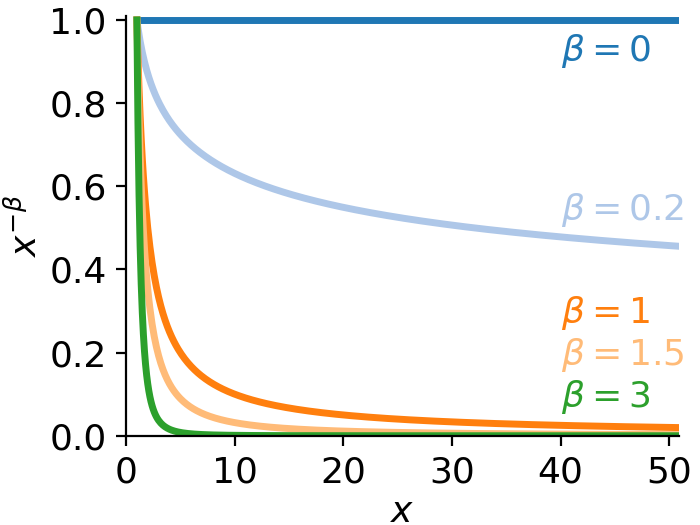
\includegraphics[scale=0.75]{images/generated/power-law}
    \caption{Power-law functions}
    \label{fig:power-law-functions}
\end{figure}

\begin{figure}
    \centering
    \subfloat{{
        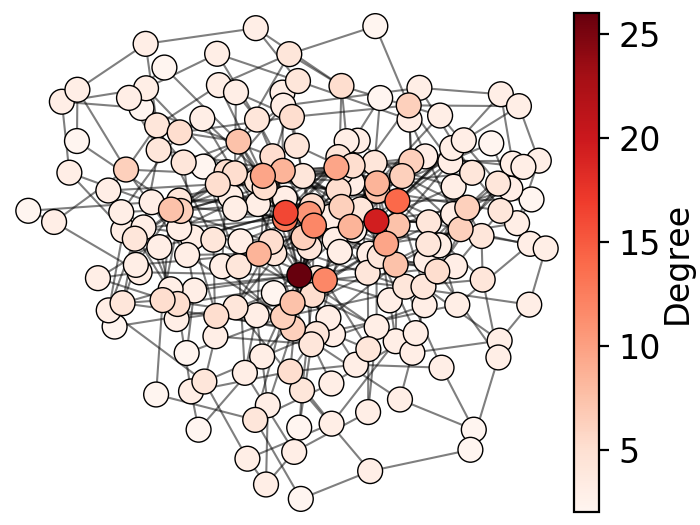
\includegraphics[scale=0.81]{images/generated/power-law-graph}
    }}
    \qquad
    \subfloat{{
        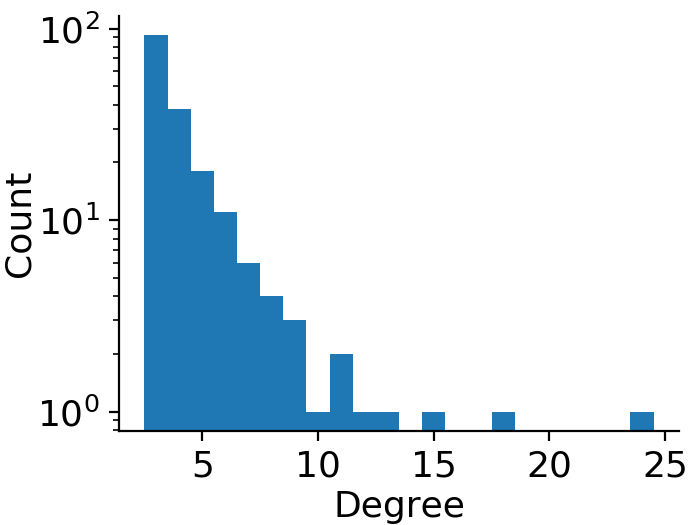
\includegraphics[scale=0.75]{images/generated/power-law-deg-distribution}
    }}
    \caption{Example of a power-law graph and its degree distribution}
    \label{fig:power-law-graph-and-deg-distr}
\end{figure}

\begin{figure}
    \centering
    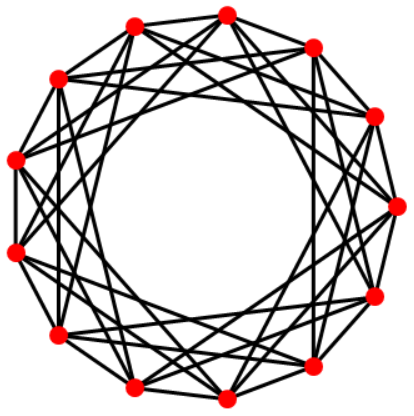
\includegraphics[width=0.35\textwidth]{images/paley}
    \caption{13-Paley graph is an example of an expander}
    \label{fig:paley-graph}
\end{figure}

\section{Related Work}

The following results inspired us to look for expanders inside power-law graphs.

Aiello, Chung, and Lu~\cite{acl01} introduced a random graph model for power-law graphs
and described different properties, including connectivity and emergence of giant connected components.
This model is asymptotically equivalent to our coin toss model from~\autoref{sec:powerlaw-coin-toss-model}.
The difference is that our model defines the expected degree sequence
rather than the exact one, and that is crucial for our proof.

Chung and Lu~\cite{cl04} found the average distance in random graphs
with given expected degree sequences, both general and power-law with $2<\beta<3$.
The latter produces the ``octopus'' graphs described in~\autoref{sec:powerlaw-octopus-model}.

Ansotegui, Bonet, and Levy~\cite{abl09} presented a power-law model which was shown to fit well
industrial SAT instances used in recent international competitions for SAT solvers.
They also focused on fitting the SAT instances,
i.e., estimating the appropriate distributions that would produce analogous degree sequences.
We talk about this model in~\autoref{sec:powerlaw-k-cnf-model}.

Krivelevich~\cite{kri17} looked for a linearly sized expanders inside graphs
that are ``locally sparse'', as well as inside random $G(n,p)$ graphs.
The paper also contained the algorithm for actually finding the expanding subgraphs.

Finally, Mihail, Saberi, and Tetali~\cite{mst06} capitalized on the structure of power-law graphs
by displaying that one can discover the nodes via a random walk
with lookahead in sublinear time.
Considering another work by Mihail~\cite{mih89}, this result also hints on possible expansion
properties of graphs with paths of constant length replaced by new edges.

As can be seen, there is a substantial amount of research done concerning separately
power-law models and expander graphs due to their wide popularity and usefulness.
Gkantsidis, Mihail, and Saberi~\cite{gms03} made significant steps
in the direction of combining these two topics.
They considered random power-law graphs with the exponent $2<\beta<3$,
degrees of vertices between $3$ and $O(\sqrt{n})$, and volume $O(n)$.
They also had to slightly modify graph construction used by Aiello et al.~\cite{acl01}
in order to ensure certain connectivity properties.
These graphs were shown to have conductance $\Theta(1)$,
which generalizes the notion of $(n/2,\Theta(1))$ edge expansion.

\begin{table}
    \begin{center}
        \caption{Comparison of power-law graph models}
        \label{tab:models-comparison}
        \renewcommand*{\arraystretch}{1.3}
        \begin{tabular}{|l|c|c|l|}
            \hline
            \multicolumn{1}{|c|}{Model} & \multicolumn{2}{|c|}{Object} & \multicolumn{1}{|c|}{Definition} \\
            \hline\hline
            Permutation model & \multirow{2}{*}{\vspace{-4mm}exact} & degrees & $\deg(i)=\frac{pn}{i^\beta}$\rule{0pt}{18pt}\\[0.6em]
            \cline{1-1}\cline{3-4}
            Model 3~\cite{acl01} & & \multirow{2}{*}{{\renewcommand{\arraystretch}{1.0}\begin{tabular}{@{}l@{}}\\frequencies\\of degrees\end{tabular}}} & $|\{i \in V\;|\;\deg(i)=x\}|=\frac{e^\alpha}{x^\beta}$\rule{0pt}{18pt}\\[0.6em]
            \cline{1-2}\cline{4-4}
            Coin toss model & \multirow{2}{*}{\vspace{-4mm}expected} & & $\E_G[|\{i \in V\;|\;\deg(i)=x\}|]=\frac{e^\alpha}{x^\beta}$\rule{0pt}{18pt}\\[0.6em]
            \cline{1-1}\cline{3-4}
            Model 4~\cite{cl04} & & degrees & $\E_G[\deg(i)]=w_i=ci^{-1/(\beta-1)},\;\beta>2$\rule{0pt}{18pt}\\[0.6em]
            \hline
        \end{tabular}
    \end{center}
\end{table}

\section{Contribution of the Thesis}

We defined the models of power-law graphs, which would complement the ones studied earlier.
\autoref{tab:models-comparison} presents their comparison.
The permutation model was chosen so as to fit the uniformly random case when the exponent $\beta=0$.

The main result is that, under these models, the subgraphs containing
the vertices of sufficiently large degrees are edge or vertex expanders w.h.p.

More precisely, in the coin toss model, if $\beta<1$, actually the whole graph is an edge expander.
For $1\leq\beta\leq 1.6$ we have a linear size expanding subgraph,
and for $\beta>1.6$ the size of the expander is only $\Theta(n^{1/\beta})$.
In all the cases edge expansion is close to one half of the expected average degree $d$,
which is linear in the size of the subgraph.

In the permutation model, the case $\beta=0$ matches the previously known fact
that the whole graph has edge and vertex expansion almost $d-2$.
When $\beta>0$, we generalize the argument to show existence
of the edge expanders of size $n/2$ with expansion $d/2$,
but the average degree $d$ deteriorates for larger $\beta$.
Also, if $\beta>1$, there is an additional constraint $p\,\zeta(\beta)>2$
which essentially limits $\beta\leq 1.72$.
Meanwhile, vertex expansion of the subgraph with vertices of degree
at least $d_0$ is almost $d_0/2-2$ whenever $\beta>0$.

Obtained results about linear size expanders inside power-law graphs
resemble existing result of the same nature for Erd\H{o}s-R\'enyi graphs~\cite{kri17}.
The size of our expanders is also comparable to the sizes of
the largest connected components in power-law graphs~\cite{acl01}, i.e.,
we say that the largest components are not just connected, but ``highly connected''.
\autoref{tab:consistency-of-results} summarizes these details.

We proceed by showing that the core of the ``octopus'' graph with the vertices
of degree at least $n^{1/\log\log n}$ is an edge expander w.h.p.
and it contains a large vertex expander.

As a side result, we prove the logarithmic diameter of vertex expanders
with only small expanding subsets of size at most $\epsilon n$, for some
constant $\epsilon>0$, as opposed to $\epsilon=1/2$ in the canonical result.

To sum up, our findings provide better understanding of the structure
of power-law graphs from some general families for a wide range of parameters.
This knowledge can be further used to employ any techniques
applicable to expanders on these power-law graphs.

\begin{table}
    \begin{center}
        \caption{Consistency of sizes between our results and the other papers}
        \label{tab:consistency-of-results}
        \renewcommand*{\arraystretch}{1.3}
        \begin{tabular}{|l|c|c|c|c|}
            \hline
            \multicolumn{1}{|r|}{$\beta$} & $(0;1.6]$ & $(1.6;1.72]$ & $(1.72;3.48)$ & $(3.48;\infty)$\\
            \hline\hline
            {\renewcommand{\arraystretch}{1.0}\begin{tabular}{@{}l@{}}The largest components\\in power-law graphs~\cite{acl01}\end{tabular}} & \multicolumn{3}{|c|}{the giant component, $\Theta(n)$} & $O\left(n^{2/\beta}\log n\right)$\rule{0pt}{19pt}\\[0.7em]
            \hline
            {\renewcommand{\arraystretch}{1.0}\begin{tabular}{@{}l@{}}Our edge expanders\\in coin toss model\end{tabular}} & $\Theta(n)$ & \multicolumn{3}{|c|}{$\Theta\left(n^{1/\beta}\right)$}\rule{0pt}{19pt}\\[0.7em]
            \hline\hline
            {\renewcommand{\arraystretch}{1.0}\begin{tabular}{@{}l@{}}Vertex/edge expanders\\in $G(n,p)$~\cite{kri17}\end{tabular}} & \multicolumn{4}{|c|}{$\Theta(n)$}\rule{0pt}{19pt}\\[0.7em]
            \hline
            {\renewcommand{\arraystretch}{1.0}\begin{tabular}{@{}l@{}}Our edge expanders\\in permutation model\end{tabular}} & \multicolumn{2}{|c|}{$\Theta(n)$} & \multicolumn{2}{|c|}{---}\rule{0pt}{19pt}\\[0.7em]
            \hline
        \end{tabular}
    \end{center}
\end{table}

\section{Our Methods}
%extra problems solved, difficulties encountered, our approach/methods/toolbox

For the coin toss model, we first obtain the necessary lower bounds
on the expected average degree. This is done by approximating
the expected size of an arbitrary cut, applying Chernoff concentration bounds,
and following the common argument for edge expansion.
Then we decide the size of an expanding subgraph and try to keep it linear
in the size of the whole graph by choosing an appropriate minimum degree
of vertices to be included in this subgraph.

While working with the permutation model, we adopt and generalize
the existing approaches from~\autoref{subsec:edge-expansion-reg}
and~\ref{subsec:vertex-expansion-reg}
for edge and vertex expansion of regular graphs.

Throughout this work, we deal with varying approximations of harmonic numbers,
so we have to treat different ranges of the exponent $\beta$ separately.
Lastly, our proof of small diameter of vertex expanders resembles
a common technique for graph decomposition.

\section{Thesis Structure}

In~\autoref{ch:prelims} we present all the necessary definitions,
approximations, and known results about expanders,
on which this research is based.
\autoref{ch:powerlaw} contains the detailed description
of the main models of power-law graphs used in this work.
In~\autoref{ch:expanders} we show the existence of expanding subgraphs
for the coin toss and permutation models,
and analyze the diameter of graphs with vertex expansion of small sets.
Finally, we compare the behavior of the random graphs
under different models in~\autoref{ch:comparison}, including their
diameters and sizes of expanders and connected components.
